\documentclass[ALICE,manyauthors]{cernphprep}

\usepackage[comma,square,numbers,sort&compress]{natbib}
\usepackage{hyperref}
\usepackage{lineno}
%\usepackage{subcaption}
\usepackage{subfigure}
\usepackage[section]{placeins}
\usepackage {multicol}% Multi column in the table
\usepackage {multirow}% Multi row in the table
\usepackage {units}
\usepackage {array}
\linenumbers

% $Id: commands.tex 934 2013-06-19 20:56:45Z mfloris $

\newcommand{\mrm}[1]{\mathrm{#1}}
\newcommand{\mrmo}[1]{\mathrm{\overline{#1}}}
\newcommand{\bsb}[1]{\boldsymbol{#1}}
\newcommand{\circit}{\item[$\circ$]}

\newcommand{\ITS}          {\rm{ITS}}
\newcommand{\TOF}          {\rm{TOF}}
\newcommand{\ZDC}          {\rm{ZDC}}
\newcommand{\ZDCs}         {\rm{ZDCs}}
\newcommand{\ZNA}          {\rm{ZNA}}
\newcommand{\ZNC}          {\rm{ZNC}}
\newcommand{\SPD}          {\rm{SPD}}
\newcommand{\SDD}          {\rm{SDD}}
\newcommand{\SSD}          {\rm{SSD}}
\newcommand{\TPC}          {\rm{TPC}}
\newcommand{\VZERO}        {\rm{VZERO}}
\newcommand{\VZEROA}       {\rm{VZERO-A}}
\newcommand{\VZEROC}       {\rm{VZERO-C}}
\newcommand{\pip}          {$\pi^{+}$}
\newcommand{\pim}          {$\pi^{-}$}
\newcommand{\kap}          {K$^{+}$}
\newcommand{\kam}          {K$^{-}$}
\newcommand{\pbar}         {$\rm\overline{p}$}
\newcommand{\kzero}        {\ensuremath{{\rm K}^{0}_{S}}}
\newcommand{\kstar}        {\ensuremath{{\rm K}^{*}}}
\newcommand{\He}           {\ensuremath{^{3}{\rm He}}}
\newcommand{\LH}           {\ensuremath{^{3}_{\Lambda}{\rm H}}}
\newcommand{\vzero}        {\ensuremath{{\rm V}^0}}
\newcommand{\lmb}          {\ensuremath{\Lambda}}
\newcommand{\almb}         {\ensuremath{\bar{\Lambda}}}
\newcommand{\allpart}      {$\pi^{\pm}$, K$^{\pm}$, \kzero, p(\pbar) and \lmb(\almb)}
\newcommand{\allpi}        {$\pi^{\pm}$}
\newcommand{\allk}         {K$^{\pm}$}
\newcommand{\allp}         {p(\pbar)}
\newcommand{\alllmb}       {\lmb(\almb)}
\newcommand{\degree}       {$^{\rm o}$}
\newcommand{\dg}           {\mbox{$^\circ$}}
\newcommand{\dedx}         {\ensuremath{\mathrm{d}E/\mathrm{d}x}}
\newcommand{\dndy}         {d$N$/d$y$}
\newcommand {\ee}            {\mbox{e$^+$e$^-$}}
\newcommand{\pp}           {pp}
\newcommand{\ppbar}        {\mbox{$\mathrm {p\overline{p}}$}}
\newcommand{\PbPb}         {\mbox{Pb--Pb}}
\newcommand{\pPb}          {\mbox{p--Pb}}
\newcommand{\AuAu}         {\mbox{Au--Au}}
\newcommand{\pseudorap}    {\mbox{$\left | \eta \right | $}}
\newcommand{\dNdeta}       {\ensuremath{\mathrm{d}N_\mathrm{ch}/\mathrm{d}\eta}}
\newcommand{\dNdy}         {\ensuremath{\mathrm{d}N/\mathrm{d}y}}
\newcommand{\dNdptdy}      {\ensuremath{\mathrm{d}N/{\rm d}\pt\mathrm{d}y}}
\newcommand{\dNdyst}       {\ensuremath{\sqrt{\frac{dN_\pi/dy}{s_T}}}}
\newcommand{\dNdetatr}     {\mathrm{d}N_\mathrm{tracklets}/\mathrm{d}\eta}
\newcommand{\dNdetar}[1]   {\mathrm{d}N_\mathrm{ch}/\mathrm{d}\eta\left.\right|_{|\eta|<#1}}
\newcommand{\lum}          {\, \mbox{${\rm cm}^{-2} {\rm s}^{-1}$}}
\newcommand{\barn}         {\, \mbox{${\rm barn}$}}
\newcommand{\m}            {\, \mbox{${\rm m}$}}
\newcommand{\ncls}         {\ensuremath{N_{cls}}}
\newcommand{\nsigma}       {\ensuremath{n\sigma}}
\newcommand{\dcaxy}        {\ensuremath{{\rm DCA}_{xy}}}
\newcommand{\dcaz}         {\ensuremath{{\rm DCA}_{z}}}
\newcommand{\EcrossB}      {E$\times$B}%{\ensuremath{{\rm E}\times{\rm B}}}
\newcommand{\bb}           {Bethe-Bloch}
\newcommand{\s}            {\ensuremath{\sqrt{s}}}
\newcommand{\pt}           {\ensuremath{p_\mathrm{T}}}
\newcommand{\pT}           {\ensuremath{p_{\rm T}}}
\newcommand{\hlab}         {\ensuremath{\eta_{\rm lab}}}
\newcommand{\ynn}         {\ensuremath{y_{\rm NN}}}
\newcommand{\ycms}         {\ensuremath{y_{\rm CMS}}}
\newcommand{\ylab}         {\ensuremath{y_{\rm lab}}}
\newcommand{\ppi}          {\ensuremath{{\rm p}/\pi}}
\newcommand{\kpi}          {\ensuremath{{\rm K}/\pi}}
\newcommand{\lpi}          {\ensuremath{{\rm \Lambda}/\pi}}
%\newcommand{\ppi}          {\ensuremath{(\pi^+ + \pi^-)/({\rm K}^+ + {\rm K}^-)}}
%\newcommand{\kpi}          {\ensuremath{({\rm p} + {\rm \bar p})/({\rm K}^+ + {\rm K}^-)}}
\newcommand{\mt}           {\ensuremath{m_{\rm T}}}
\newcommand{\snn}          {\ensuremath{\sqrt{s_{\rm NN}}}}
\newcommand{\snnbf}        {\ensuremath{\mathbf{{\sqrt{s_{\mathbf NN}}}}}}
\newcommand{\sonly}        {\ensuremath{\sqrt{s}}}
\newcommand{\Npart}        {\ensuremath{N_\mathrm{part}}}
\newcommand{\avNpart}      {\ensuremath{\langle N_\mathrm{part} \rangle}}
\newcommand{\avNpartdata}  {\ensuremath{\langle N_\mathrm{part}^{\rm data} \rangle}}
\newcommand{\Ncoll}        {\ensuremath{N_\mathrm{coll}}}
\newcommand{\Dnpart}       {\ensuremath{D\left(\Npart\right)}}
\newcommand{\DnpartExp}    {\ensuremath{D_{\rm exp}\left(\Npart\right)}}
\newcommand{\dNdetapt}     {\ensuremath{\dNdeta\,/\left(0.5\Npart\right)}}
\newcommand{\dNdetaptr}[1] {\ensuremath{\dNdetar{#1}\,/\left(0.5\Npart\right)}}
\newcommand{\dNdetape}     {\left(\ensuremath{\dNdeta\right)/\left(\avNpart/2\right)}}
\newcommand{\dNdetaper}[1] {\ensuremath{\dNdetar{#1}\,/\left(\avNpart/2\right)}}
\newcommand{\dndydpt}      {\ensuremath{{\rm d}^2N/({\rm d}y {\rm d}p_{\rm t})}}
\newcommand{\abs}[1]       {\ensuremath{\left|#1\right|}}
\newcommand{\signn}        {\ensuremath{\sigma^{\rm inel.}_{\rm NN}}}
\newcommand{\vz}           {\ensuremath{V_{z}}}
\newcommand{\Tfo}          {\ensuremath{{T}_{\rm kin}}}
\newcommand{\Tch}          {\ensuremath{{T}_{\rm ch}}}
\newcommand{\bT}           {\ensuremath{\beta_{\rm T}}}
\newcommand{\avbT}         {\ensuremath{\left< \beta_{\rm T}\right>}}
\newcommand{\avpT}         {\ensuremath{\left< \pt \right>}}
\newcommand{\muB}          {\ensuremath{\mu_{B}}}
\newcommand{\stat}         {({\it stat.})}
\newcommand{\syst}         {({\it sys.})}
\newcommand{\Fig}[1]       {Fig.~\ref{#1}}
\newcommand{\Figure}[1]    {Figure~\ref{#1}}
%\newcommand{\Ref}[1]       {Ref.~\cite{#1}}
%\newcommand{\green}[1]     {\textcolor{green}{#1}}
%\newcommand{\blue}[1]      {\textcolor{blue}{#1}}
%\newcommand{\red}[1]       {\textcolor{red}{#1}}
%\newcommand{\white}[1]     {\textcolor{white}{#1}}
\newcommand{\gevc}         {\ensuremath{{\rm GeV}/c}}
\newcommand{\mevc}         {\ensuremath{{\rm MeV}/c}}
\newcommand{\gs}           {\ensuremath{\gamma_{s}}}
\newcommand{\gq}           {\ensuremath{\gamma_{q}}}
\newcommand{\gc}           {\ensuremath{\gamma_{c}}}
\newcommand{\chindf}       {\ensuremath{\chi^{2}/{\rm NDF}}}
\newcommand{\avg}[1]       {\ensuremath{\left\langle#1\right\rangle}}
\newcommand{\etalab}       {\ensuremath{\eta_{{\rm lab}}}}
\newcommand {\gammas}			{\ensuremath{\gamma_{\mathrm{s}}}}

\newcommand{\DNDETAINEL}{5.31~$\pm$~0.18\xspace}
\newcommand{\DNDETAINELGTZERO}{6.46~$\pm$~0.19\xspace}
\newcommand{\DNDETAINELGTZEROONE}{6.61~$\pm$~0.20\xspace}

\newcommand{\inelgtzero}{INEL$>$0\xspace}
\newcommand{\average}[1]{\ensuremath{\langle #1 \rangle}\xspace}
\newcommand{\mpt}        {\ensuremath{\langle\pt\rangle}\xspace}
\newcommand{\nch}        {\ensuremath{N_\mathrm{ch}}\xspace}
\newcommand{\mnch}      {\ensuremath{\langle\nch\rangle}\xspace}
\newcommand{\nchacc}        {\ensuremath{N_\mathrm{ch}^\mathrm{acc}}\xspace}
\newcommand{\mnchacc}      {\ensuremath{\langle\nchacc\rangle}\xspace}
\newcommand{\inelg}     {\ensuremath{\mathrm{INEL}_{>0}}}



\newcommand{\dndeta}{\ensuremath{{\rm d}N_{\rm ch}/{\rm d}\eta}\xspace}
\newcommand{\dndpt}{\ensuremath{{\rm d}N_{\rm ch}/{\rm d}\pt}\xspace}
\newcommand{\etaless}[1]{\ensuremath{\left|\eta\right| < #1}\xspace}
\newcommand{\dndetaless}[1]{\ensuremath{{\rm d}N_{\rm ch}/{\rm d}\eta|_{\etaless{#1}}}\xspace}
\newcommand{\avdndeta}{\ensuremath{\langle \dndeta \rangle}}
\newcommand{\zvtx}{\ensuremath{z_\mathrm{vtx}}}
\newcommand{\pythiae}{\ensuremath{\mathrm{PYTHIA}\,8}}
%\newcommand{\pythiam}{\ensuremath{\mathrm{PYTHIA}\,8\,\mathrm{Monash}\,2013}}
\newcommand{\pythiam}{\ensuremath{\mathrm{PYTHIA}\,8\,\mathrm{Tune\,4C}}}
\newcommand{\pythiashoving}{{\ensuremath{\mathrm{PYTHIA}\,8~\mathrm{String}~}}\ensuremath{\mathrm{Shoving}}}
\newcommand{\epos}{{\ensuremath{\mathrm{EPOS}\,~\mathrm{LHC}}}}
%\newcommand{\pythiashoving}{\ensuremath{\mathrm{PYTHIA}\,8~\mathrm{String}~}\linenomath{-}\ensuremath{\mathrm{Shoving}}}
\newcommand{\pttrig}{\ensuremath{p_\mathrm{T,\,trig}}}
\newcommand{\ptassoc}{\ensuremath{p_\mathrm{T,\,assoc}}}
\newcommand{\ptjet}{\ensuremath{p_\mathrm{T,\,jet}^\mathrm{ch}}}
\newcommand{\ptlead}{\ensuremath{p_\mathrm{T,\,LP}}}
\newcommand{\pttrigassoc}{\ensuremath{p_\mathrm{T,\,trig\,(assoc)}}}









\renewcommand{\labelitemi} {$-$}
%==========================================================%
%%% inline warnings for internal discussion
%\newcommand{\warn}[1]      {\textbf{\textcolor{red}{[#1]}}}
\newcommand{\warn}[1]      {{\small\textbf{\textcolor{red}{(!\footnote{\textbf{(!)}~#1})}}}}
\newcommand{\warnin}[1]         {\textit{\textcolor{red}{(#1)}}}
%\newcommand{\warn}[1]      {#1}
%\newcommand{\warn}[1]      {{\small\textbf{(!\footnote{\textbf{(!)}~#1})}}\marginpar{\textbf{---}}}
\newcommand{\todo}[1]      {\textbf{\textcolor{red}{[TODO: #1]}}}
%%% fake numbers
\newcommand{\fake}[1]      {\textbf{\textcolor{red}{#1}}}
%\newcommand{\fake}[1]      {#1}
\newcommand{\final}[1]     {\textbf{\textcolor{blue}{#1}}}
\newcommand{\prelim}[1]    {\textbf{\textcolor{magenta}{#1}}}
\renewcommand{\mod}[1]       {\textbf{\textcolor{red}{#1}}}

\begin{document}

%%%%%%%%%%%%%%%  Title page %%%%%%%%%%%%%%%%%%%%%%%%
\begin{titlepage}

\PHyear{}
\PHnumber{2019-xxx}      % required, will be obtained from PH
%\PHdate{Day Month}  % required, will be obtained from PH
\PHdate{\today}
%

%%% Put your own title + short title here:
\title{Long- and short-range correlations and their event scale dependence in high-multiplicity pp collisions at $\sqrt{s} = 13$~TeV}
\ShortTitle{Long-range correlations in pp collisions}   % appears on right page headers

%%% Do not change the next lines
%\Collaboration{ALICE Collaboration\thanks{See Appendix~\ref{app:collab} for the list of collaboration members}}
\ShortAuthor{ALICE Collaboration} % appears on left page headers, do not change

\begin{abstract}
%The observed azimuthal modulations of long-range correlations in pseudorapidity in small systems like pp or p-Pb collisions show strikingly similar features to those seen in heavy ion collisions. Many theoretical approaches to interpreting this effect have been developed. However, it is still unclear whether these long-range correlations are due to final or initial state effects. To further investigate these effects, we studied long-range correlations as a function of transverse momentum in very high multiplicity pp collisions at $\sqrt{s} =13$ TeV, collected with the high multiplicity event trigger during 2016 and 2017 with ALICE. In this talk, we present the near-side per-trigger yield at large pseudorapidity separation (ridge yield) as a function of transverse momentum in pp collisions at $\sqrt{s} =13$ TeV. The results are compared to previous measurements from CMS experiments. In addition, we present the ridge yield in events where harder fragmentation processes are present, to explore possible physical origins of long-range correlations.


Two-particle angular correlations have been measured in high-multiplicity $\sqrt{s} =13$ TeV proton-proton collisions by the ALICE collaboration. From the correlations, the yields of particle pairs at short-($\Delta\eta$ $\sim$ 0) and long-range ($1.6 < |\Delta\eta| < 1.8$) in rapidity have been extracted on the near side ($\Delta\varphi$ $\sim$ 0).
The correlations and yields are reported as a function of transverse momentum ($p_{\mathrm T}$) in the range 1$ < p_{\mathrm T} < $4 GeV/$c$.
Furthermore, the event-scale dependence has for the first time been studied by requiring the presence of high-$p_{\rm T}$ leading tracks and/or jets for varying $p_{\rm T}$ thresholds. 
The results demonstrate that the long-range ``ridge`` yield, related to the collective behavior of the produced system, is present in events with high-$p_{\mathrm T}$ processes. The magnitudes of the short- and long-range yields are found to grow with the event scale. 
The results have been compared to calculations with EPOS LHC and PYTHIA 8, with and without string-shoving interactions. It is found that while both models describe the qualitative trends in the data, EPOS LHC shows a better quantitative agreement, in particular for the $p_{\rm T}$ and event scale dependencies.

%Long-range azimuthal correlations are measured in high-multiplicity pp collisions at center-of-mass energy $\sqrt{s} = 13$~TeV by the ALICE collaboration at the LHC. The measurement was carried out for trigger and associated particles having transverse momenta in the range $1 < p_{\mathrm T} < 5$~GeV/$c$. Trigger and associated particles were separated by a large pseudorapidity interval $1.6 < |\Delta \eta |<1.8$. Measured ridge yield is consistent with the results from the CMS collaboration.
%These resfults are obtained in a relative pseudorapidity range of $1.6 < |\eta| < 1.8$ and transverse momentum region of  for the trigger and associated particles.
%In addition to the conventional long-range correlation studies, the results are further investigated in events with a high-$p_{\rm{T}}$ leading track or jet.
%where jets with a harder fragmentation are present.
%The jets are reconstructed by using the anti-$k_\mathrm{T}$ algorithm with resolution parameter $R=0.4$ in $|\eta_\mathrm{jet}|<0.4$. 
%The magnitude of the correlation dubbed ridge yield, is consistent with the results from other LHC experiments for unbiased events.
%These long-range correlations are also seen in the events containing high-$\pt$ jets for the first time. Furthermore, data show that the ridge yield tends to grow with transverse momentum of the jet or leading track. %increase in events holding $\ptjet > 10$~GeV/$c$.
%Event-scale selection is further studied by measuring the near-side jet-like peak.
%The results are compared to $\pythiashoving$ and $\epos$ calculations.  
%$\pythiashoving$ model can describe low $p_{\mathrm T}$ ridge yields up to 1.5 GeV/$c$ but can not give a good description of $p_{\mathrm T}$ dependence both for the unbiased and jet-tagged events. $\epos$ model can describe $\pt$ dependence of ridge yield while overestimating the yield at the low $\pt<$ 2 GeV/$c$. On the other hand, near-side jet-like correlations are overestimated by $\pythiashoving$ and quantitatively estimated by $\epos$, which is opposite description to the ridge yield.


\end{abstract}

\end{titlepage}

\setcounter{page}{2}

\section{Introduction}

%Studies of particle correlations in high-energy hadronhadron collisions provide valuable information on the underlying quantum chromodynamics processes leading to particle production. Measurements of two-particle angular correlations are typically performed in terms of twodimensional Δη-Δϕ correlation functions, where η is the pseudorapidity and ϕ is the azimuthal angle. Of particular interest in studies of possible novel partonic collective effects is the long-range (e.g., jΔηj > 2.0) structure of twoparticle correlation functions, in which the effects of known sources such as resonance decays and fragmentation of high-momentum partons are known to be small. In most Monte Carlo (MC) event generators for proton-proton (pp) collisions, the typical sources of such long-range correlations are momentum conservation and away-side (Δϕ ≈ π) jet correlations. Measurements in high-energy nucleusnucleus collisions have shown a long-range structure in the two-particle angular correlations functions, which has been attributed to the presence of the hot and dense matter formed [1]. Several novel features were observed in azimuthal correlations over large Δη for intermediate particle transverse momenta, pT ≈ 1–5 GeV=c [2,3]. These correlations are thought to arise from the response of a hydrodynamically expanding partonic medium to fluctuations of the initial collision geometry [4–9]. Measurements in pp collisions at a center-of-mass energy of ffiffi s p ¼ 7 TeV have also revealed the presence of long-range, near-side (Δϕ ≈ 0) correlations in events with very large final-state particle multiplicity [10]. Similar phenomena have also been observed in high-multiplicity proton-lead (pPb) collisions [11–13], where they have been studied extensively [14–21]. A wide range of models have been suggested to explain the emergence of these correlations in pp [22] and pPb [23–27] collisions. While models based on a hydrodynamic approach can describe many aspects of the observed correlations [23,24], it has been proposed that initial-state correlations of gluon fields could also lead to similar effects [25–27].

%Two-particle correlations are a powerful tool to explore the mechanism of particle production in collisions of hadrons and nu-clei at high energy. Such studies involve measuring the distribu-tions of relative anglesφandηbetween pairs of particles: a“trigger” particle in a certain transverse momentumpT,trigintervaland an “associated” particle in apT,associnterval, whereφandηare the differences in azimuthal angleφand pseudorapidityηbetween the two particles.In proton–proton (pp) collisions, the correlation at (φ≈0,η≈0) forpT,trig>2GeV/cis dominated by the “near-side” jetpeak, where trigger and associated particles originate from a frag-menting parton, and atφ≈πby the recoil or “away-side” jet[1].The away-side structure is elongated alongηdue to the longitu-dinal momentum distribution of partons in the colliding protons.In nucleus–nucleus collisions, the jet-related correlations are mod-ified and additional structures emerge, which persist over a longrange inηon the near side and on the away side[2–14].Theshape of these distributions when decomposed into a Fourier se-ries defined byvncoefficients[15]is found to be dominated bycontributions from terms withn=2 andn=3 [6,7,9–14].Thevncoefficients are sensitive to the geometry of the initial stateof the colliding nuclei[16,17]and can be related to the transport properties of the strongly-interacting de-confined matter via hy-drodynamic models[18–20].Recently, measurements in pp collisions at a centre-of-massenergy√s=7TeV[21]and in proton–lead (p–Pb) collisions ata nucleon–nucleon centre-of-mass energy√sNN=5.02 TeV[22]have revealed long-range (2<|η|<4) near-side (φ≈0) cor-relations in events with significantly higher-than-average particlemultiplicity. Various mechanisms have been proposed to explainthe origin of these ridge-like correlations in high-multiplicity ppand p–Pb events. These mechanisms include colour connectionsforming along the longitudinal direction[23–26], jet-medium[27]and multi-parton induced[28,29]interactions, and collective ef-fects arising in the high-density system possibly formed in thesecollisions[30–35].Results from two-particle correlations in√sNN=0.2TeVd–Aucollisions[36,37]show a strong suppression of the away-side yieldat forward rapidity in central collisions. This modification has beeninterpreted in the framework of “Colour Glass Condensate” mod-els [38]as a saturation effect caused by nonlinear gluon inter-actions in the high-density regime at small longitudinal partonmomentum fractionx. Similar effects may arise at midrapidity inp–Pb collisions at√sNN=5.02 TeV, where the parton distributionsare probed down tox<10−3, which is comparable to the relevantrange ofxat forward rapidity (y∼3) at√sNN=0.2TeV.This Letter presents results extracted from two-particle cor-relation measurements in p–Pb collisions at√sNN=5.02 TeV,recorded with the ALICE detector[39]at the Large Hadron Col-lider (LHC). The correlations are measured over two units of pseudorapidity and full azimuthal angle as a function of charged-particle multiplicity, and expressed as associated yield per triggerparticle. Sections2 and 3describe the experimental setup, andthe event and track selection, respectively. Details on the defini-tion of the correlation and the per-trigger-particle associated yieldare given in Section4. The results of the analysis are discussed inSection5 and a summary is given in Section


Collective effects are one of the key probes to study evolution of the hot and dense matter created in ultra-relativistic heavy-ion collisions. The enhancement in the associated yield of two-particle correlations at small relative azimuthal angle ($\Delta\varphi$) that extends over a long-range of relative pseudorapidity ($\Delta\eta$), often referred to as the “ridge”,  is one of the crucial observables of collectivity \cite{ridge_aa_1, ridge_aa_2}. In recent years, measurements of the ridge in small systems, such as proton-proton (pp) collisions and proton-nucleus (pA) collisions, where the volume and lifetime of the medium produced are expected to be small, have been reported\cite{ridge_pp_1, ridge_pp_2, ridge_pp_3, ridge_pp_4}. There are many theoretical attempts\cite{ridge_theory_1, ridge_theory_2, ridge_theory_3, ridge_theory_4} to interpret the ridge considering hydrodynamics, saturation or other mechanisms, but a quantitative description of the full set of experimental data has not yet been achieved.




%Measurements of two-particle angular correlations in high-multiplicity proton-proton (pp) collisions at a centerof-mass energy ffiffi s p ¼ 7 TeV at the LHC showed an enhancement in the production of pairs at small azimuthal-angle separation, Δϕ, that extends over a wide range of pseudorapidity differences, Δη, and which is often referred to as the “ridge” [1]. The ridge has also been observed in proton-lead (p þ Pb) collisions [2–7], where it is found to result from a global sinusoidal modulation of the per-event single-particle azimuthal angle distributions [3–6]. While many theoretical interpretations of the ridge, including those based on hydrodynamics [8–12], saturation [13–23], or other mechanisms [24–30], have been, or could be applied to both pp and p þ Pb collisions, it has not yet been demonstrated that the ridge in pp collisions results from single-particle azimuthal anisotropies. Testing whether the ridges in pp and p þ Pb collisions arise from the same underlying features of the single-particle distributions may provide insight into the physics responsible for the phenomena. Separately, a study of the ffiffi s p dependence
%Collective effect is one of key probes to explore evolution of the hot and dense matter as consequence of heavy ion collisions at high energy. One novel tool for studying the collective effect is two-particle angular correlations as function of relative pseudo-rapidity($\Delta\eta$) and azimuthal angle($\Delta\varphi$) between the trigger particle and the associated particle. The main source of collective

%QCD has been studied through particles produced in heavy ion collisions. Among many observables, collective effect is one of key probes to explore evolution of the hot and dense matter as results of heavy ion collisions. One novel tool to study the initial conditions and their evolution is angular correlations of two-particle with respect to two-dimensional $\Delta\eta-\Delta\varphi$ distribution, Where $\eta$ denotes pseudorapidity and $\varphi$ denotes azimuthal angle. Especially, much interest.in the distribution is with long-range $\Delta\eta$, where the collective effect thought to be dominant. 




\section{Experimental setup}
\label{sec:experiment}

%LHC at CERN produces various interesting phenomena including the ridge effect that is the main topic of the document in pp collisions with the highest center-of-mass energy in the world.
%Recent center-of-mass energy in pp collisions reaches up to $\sqrt{s} = 13$~TeV during the last LHC Run 2 period. 
The analysis is based on the data sets of pp collisions at $\sqrt{s} = 13$~TeV collected from 2016 to 2018 during the LHC Run 2 period. The full description of the ALICE detector in the LHC Run 2 can be found in Refs.~\cite{Aamodt:2008zz,Abelev:2014ffa}. The present analysis mainly utilizes the V0~\cite{Abbas:2013taa}, ITS (Inner Tracking System)~\cite{aliceITS}, and TPC (Time Projection Chamber)~\cite{aliceTPC} detectors.

The V0 detector consists of two rings, V0-A and V0-C, each made of 32 scintillator tiles, covering the full azimuthal angle within the pseudorapidity intervals $2.8 < \eta < 5.1$ and $-3.7 < \eta < -1.7$, respectively. 
The V0 is used to assess event activity and it provides minimum bias (MB) and high-multiplicity (HM) trigger. The minimum bias trigger is obtained by a time coincidence of V0A and V0C signals. The high multiplicity trigger requires that amplitude of the combined V0A and V0C signal exceeds 5 times the mean value measured in minimum bias collisions, providing top 0.1\% events of MB events.

Charged particles are reconstructed by the ITS and TPC, which are working in a uniform solenoidal magnetic field of 0.5~T. The ITS is composed of three sub-systems, Silicon Pixel Detector (SPD), Silicon Drift Detector (SDD), and Silicon Strip Detector (SSD). You can find more details about SPD in~\cite{Santoro2009:ALICESPD}. The ITS and TPC covering the full azimuthal region have acceptances up to $|\eta| < 1.4$ and 0.9, respectively, for detection of charged particles with a primary vertex in $|z_\mathrm{vtx}| < 8$~cm. The tracking of charged particles is done with the combined information of the ITS and TPC that enables the reconstruction of tracks down to 0.15~GeV/$c$ with about 65\% efficiency. The efficiency goes up to 80\% for intermediate transverse momentum, 1--5~GeV/$c$. The transverse momentum resolution is around 1\% for primary tracks with low $\pt<$1~GeV/$c$, and linearly degrades up to 6\% at $\pt \sim$ 40~GeV/$c$~\cite{Contin_2012:ITSPTRES}.
%https://arxiv.org/pdf/1910.14400.pdf
%https://arxiv.org/abs/1402.4476


\section{Analysis Procedure}
\label{sec:ana}

The analyzed data samples of minimum-bias and high-multiplicity pp $\sqrt{s}=$13 TeV events correspond to integrated luminosities of 19 nb$^{-1}$ and 11.4 pb$^{-1}$, respectively~\cite{ALICE-PUBLIC-2016-002}.

The primary vertex position is reconstructed by combining observed signal clusters in the SPD. Reconstructed primary vertices of selected events are required to be located within 8 cm from the ALICE center. Probability of pileup events is about 0.6\%. Pileup events can be resolved and rejected if the longitudinal displacement of their primary vertices is larger than 0.8 cm. The probability of pileup is estimated to be 0.6\%.

%Requirements for reconstruction of charged particles are optimized to have the flat angular distribution of charged particles that is called hybrid tracks to minimize the effect of inactive regions of the ITS and TPC detectors~\cite{hybridExplanation}.  The hybrid tracks combine two different classes of tracks. The first class consists of tracks that have at least one hit in the SPD. The tracks from the second class do not have any SPD associated hit and mainly rely on the position information of the primary vertex when reconstructing the tracks.
Charge particle selection criteria are optimized for a homogeneous response over the full TPC volume to mitigate the effect of small regions where some of ITS layers are inactive. The selected set of tracks consists of two track classes. Tracks from the first class are required to have at least one hit in the SPD. Tracks from the second class do not have any SPD associated hit and their initial point is instead constrained to the primary vertex.

The two-particle correlations function is measured as a function of relative pseudorapidity ($\Delta\eta$) and azimuthal angle differences ($\Delta\varphi$) between the trigger and associated particles,
\begin{eqnarray}
\frac{1}{N_{\rm{trig}}} \frac{ \rm{d}\it{}^{2} N_{\rm{pair}} }{ \rm{d} \Delta\eta \rm{d}\Delta\varphi} = B(0, 0)\frac{S(\Delta\eta, \Delta\varphi)}{B(\Delta\eta, \Delta\varphi)}  \lvert_{\pttrig,\ptassoc}   \quad.
\label{eq:corrfunction}
\end{eqnarray}
where $\pttrig$ and $\ptassoc$ are transverse momenta of the trigger and associated particles, respectively, $N_\mathrm{trig}$ is the number of trigger particles and $N_\mathrm{pair}$ is the number of trigger-associated particle pairs. $N_\mathrm{trig}$ and $N_\mathrm{pair}$ were corrected for track reconstruction efficiencies as $N_\mathrm{trig,cor} = N_\mathrm{trig}/ \epsilon_{\rm{trig}}$ and $N_\mathrm{pair,cor} = N_\mathrm{pair}/(\epsilon_{\rm{trig}}\epsilon_{\rm{assoc}})$ for a given $\pt$ and $\eta$, respectively. 
$S (\Delta\eta, \Delta\varphi)$ is constructed using two-particle correlations in the same event and $B(\Delta\eta, \Delta\varphi)$ in mixed events. $B(\Delta\eta, \Delta\varphi)$ is normalized by its value at $\Delta\eta$ and $\Delta\varphi = 0$, represented as $B (0,0)$. Primary vertices of events to be mixed are required to be within the same, 2 cm wide $z_{vtx}$ bin. The final per-trigger yield is constructed by averaging correlation functions over these primary vertex bins.

Ridge yields at large $\Delta\eta$ are extracted for various multiplicity classes and transverse momentum intervals. The large $\Delta\eta$ range is selected as $1.6<|\Delta\eta|<1.8$, where non-flow effects (mainly coming from jets) are negligible on the near-side. In this region, the $\Delta\varphi$ distribution, or the so called per-trigger yield is expressed as
\begin{eqnarray}
\frac{1}{N_{\rm{trig}}} \frac{ \rm{d}\it{}N_{\rm{pair}} }{ \rm{d}\Delta\varphi } = \int_{1.6<|\Delta \eta|<1.8} \rm{d} \Delta \eta \left( \frac{1}{\it{N}_{\rm{trig}}} \frac{ \rm{d}\it{}^{2} N_{\rm{pair}} }{ \rm{d}\Delta\eta d\Delta\varphi} \right) \dfrac{1}{\delta\Delta\eta} \quad.
\end{eqnarray}

The baseline of the correlations is subtracted by means of the Zero-Yield-At-Minimum (ZYAM) procedure~\cite{Ajitanand:2005jj}. The minimum yield $(C_{\rm{ZYAM}})$ at the $\Delta\varphi=\Delta\varphi_{\rm{min}}$ in the $\Delta\varphi$ projection (Note that the value of $\Delta\varphi_{\rm{min}}$ can be different in data and in models.) is obtained from the function, which fits the data with a Fourier series up to the third harmonic. Subtracting $C_{\rm{ZYAM}}$ from the $\Delta\varphi$ projection makes the yield at $\Delta\varphi_{\rm{min}}$ zero. The ridge yield ($Y^{\rm{ridge}}$) is obtained by integrating the near-side peak of the $\Delta\varphi$ projection over $|\Delta\varphi|<|\Delta\varphi_{\rm{min}}|$ after the ZYAM procedure,
\begin{eqnarray}
Y^{\rm{ridge}} = \int_{|\Delta \varphi| < |\Delta\varphi_{\rm{min}}| } \rm{d} \Delta\varphi \frac{1}{\it{N}_{\rm{trig}}} \frac{ \rm{d}\it{}N_{\rm{pair}} }{ \rm{d}\Delta\varphi } \quad.
\end{eqnarray}

The ridge yield is further studied in events having a hard jet or a high-$\pt$ leading particle in the mid rapidity. Such requirement is expected to bias impact parameter of pp collisions to be smaller on average~\cite{Sjostrand:1986ep,Frankfurt:2010ea}.
%The ridge yield is further studied by exploiting the largest momentum transfer among the initial partons in a given event, which results from the hard scattering. In this article, larger momentum transfer denotes harder event-scale. The larger momentum transfer is also expected to be connected with the shorter impact parameters in pp collisions in average~\cite{Sjostrand:1986ep,Frankfurt:2010ea} so that the event-scale can be indirectly connected with the impact parameters.
% The ridge yield is further studied by exploiting the momentum transfer between the interacting partons,so called, event scale.  On average, increasingly hard parton interactions result from pp collisions with decreasing impact parameters between the two proton ///original version
The event-scale is set by requiring a minimum transverse momentum of leading track or reconstructed jet in mid-rapidity. The leading track is selected within $|\eta|<0.9$ and the full azimuthal angle. Jets are reconstructed with charged particles only (track-based jets) with the anti-$k_{\rm{T}}$ algorithm~\cite{Cacciari2008:FASTJET,Cacciari2012:FASTJET} and the resolution parameter $R=$~0.4. The recombination scheme used in this article is $\pt$ scheme. Jets are selected in $|\eta_\mathrm{jet}|<0.4$ and the full azimuthal angle. The transverse momentum of jets $p_\mathrm{T,\,jet}$ is corrected for underlying event density that is measured using the $k_{\rm{T}}$ algorithm with $R=$~0.2~\cite{ALICE2019:KTJETSub}. 

To quantify variation of near-side jet-like peak with event-scale selections using minimum $p_\mathrm{T,\,LP}$ or $p_\mathrm{T,\,jet}$, neat-side jet-like peak is extracted from near-side $\Delta\eta$ correlations. The near-side is defined as $|\Delta\varphi|<$1.28, where the correlations function is projected along to $\Delta\varphi$ direction for 1$<\pttrig$, $\ptassoc<$2 GeV/$c$ in high-multiplicity events. The near-side $\Delta\eta$ correlations are constructed as
\begin{eqnarray}
\frac{1}{N_{\rm{trig}}} \frac{ \rm{d}\it{}N_{\rm{pair}} }{ \rm{d}\Delta\eta } = \int_{|\Delta \varphi|<1.28} \rm{d} \Delta \varphi \left( \frac{1}{\it{N}_{\rm{trig}}} \frac{ \rm{d}\it{}^{2} N_{\rm{pair}} }{ \rm{d}\Delta\eta d\Delta\varphi} \right) \dfrac{1}{\delta\Delta\varphi} \quad. 
\end{eqnarray}

The baseline of the $\Delta\eta$ correlations is also subtracted by using the ZYAM procedure. The minimum yield $(C_{\rm{ZYAM}})$ of $\Delta\eta$ correlations is found within $|\Delta\eta|<$1.6 and used for subtraction from  $\Delta\eta$ correlations, which results in zero-yield at minimum. The near-side jet-like peak yield ($Y^{\mathrm{near}}$) is measured by integrating the $\Delta\eta$ correlations over $|\Delta\eta|<$1.6,
\begin{eqnarray}
Y^{\rm{near}} = \int_{|\Delta \eta|<1.6} \rm{d} \Delta\eta \left( \frac{1}{\it{N}_{\rm{trig}}} \frac{ \rm{d}\it{}N_{\rm{pair}} }{ \rm{d}\Delta\eta } - C_{\rm{ZYAM}} \right)\quad.
\end{eqnarray}

%Monte Carlo simulation with $\pythiam$ event generator and particle transport inside ALICE using GEANT3~\cite{Brun:1994aa} is used to correct the acceptance and the efficiency of the ALICE detectors. 

%The corrections have been tested by comparing the distributions, which are constructed with generated true particles and reconstructed particles with detector responses. The several percentage of non-closure has been considered into systematic uncertainty.

\section{Systematic Uncertainties of the Measured Yields}
\label{sec:uncertainties}

Systematic uncertainties on $Y^{\rm{ridge}}$ and $Y^{\rm{near}}$ were estimated by varying the analysis selection criteria and corrections and evaluated as functions of $\pttrig$($\ptassoc$) and $\ptlead$ or $\ptjet$ as described in Tab.~\ref{tab:syst}. $Y^{\rm{ridge}}(\pttrig,\,\ptassoc)$ denotes the ridge yield as a function of $\pttrig$($\ptassoc$) in event-scale unbiased events. Ridge yields measured in event-scaled biased events are denoted $Y^{\rm{ridge}}(\ptlead)$ and $Y^{\rm{ridge}}(\ptjet)$ and they were evaluated for 1$<\pttrig, \ptassoc<$2 GeV/$c$. The uncertainties on $Y^{\rm{near}}(\ptlead)$ and $Y^{\rm{near}}(\ptjet)$ were evaluated and reported in Tab.~\ref{tab:syst} together because the measured uncertainties are comparable to each other.

\begin{table}[h!]
\caption{The relative systematic uncertainty on the associated yield spectrum estimated for $Y^{\rm{ridge}}(\pttrig,\,\ptassoc)$, $Y^{\rm{ridge}}(\ptlead)$, $Y^{\rm{ridge}}(\ptjet)$, and, $Y^{\rm{near}}$, respectively.}
\centering
\begin{tabular}{|c|c|c|c|c|}
\hline 
\multirow{2}{*}{Sources}  & \multicolumn{4}{c|}{Systematic uncertainty (\%)} \\\cline{2-5} 
         & $Y^{\rm{ridge}}(\it{p}_{\rm{T, trig}},\,\it{p}_{\rm{T, assoc}})$ & $Y^{\rm{ridge}}(\it{p}_{\rm{T, Lead}})$ & $Y^{\rm{ridge}}(\it{p}_{\rm{T, Jet}})$ & $Y^{\rm{near}}$ \\ \hline \hline
Pileup rejection		& 0.8	&0.1--3.7		&0.1--3.9	&0.2--2.2	\\ \hline
Primary vertex		& 2.4	&0.5--12.2	&0.5--8.2	&1.1--7.8	\\ \hline

Tracking			& 4.0 	&2.0		&2.0	&1.5--3.4	\\ \hline

ZYAM			& 5.1	&2.1		&2.1	&N.A.	\\ \hline
Jet contamination	& 4.5	&3.4--8.1		&3.4--9.4	&N.A.	\\ \hline

Event mixing			& 4.4	&1.0--9.6		&1.0--16.4	&0.5-1.7	\\ \hline

Efficiency correction	& 2.5 	&1.2		&1.2	&3.1	\\ \hline \hline
Total(in quadrature)			& 9.7	&4.2--18.2	&4.2--22.0	&3.9--10.9 \\ 
\hline 
\end{tabular}
\label{tab:syst}
\end{table}

The uncertainty from the pileup rejection is estimated by measuring the changes of results with different rejection criteria from the default one. The multiplicity of the track contributors to each vertex determines whether the event is contaminated by pileup or not. The variation is set by the minimum multiplicity of track contributors from 5 to 3. The estimated uncertainty is 0.8\% for events without event-scale bias. The uncertainty varies up to 3.9\% for events with the $\ptlead$ or $\ptjet$ selection. The corresponding uncertainty on $Y^{\rm{near}}$ is 0.2–-2.2\%.
%Pileup cut (multbins) -> (default pileup from the physics selection)
%Pileup cut (multbins) -> PileupMV (?)

The uncertainty from the primary vertex selection along the beam axis is estimated by varying the selection range of primary vertex from $|z_\mathrm{vtx}|<$ 8 to 6 cm. The narrower primary vertex selection allows one to test the acceptance effect on the measurement. The estimated uncertainty is 0.5--12.2\% with the varying event-scale selections. The uncertainty for $Y^{\rm{near}}$ is estimated to be 1.1--7.8\%.

The uncertainty from the track selection is estimated by varying from the hybrid tracks to the other one optimized for particle identification that is called the global tracks. The selection criteria of the global tracks are almost identical to the hybrid tracks. Each global track is required to have at least one SPD hit. 
%except for the requirement of at least one hit on the SPD.
Due to the requirement, the quality of the global tracks is sensitive to the condition of the SPD, finally resulting in a non-flat azimuthal distribution of charged particles with the selection. 
%The variation is achieved by changing the mandatory SPD requirement and the maximal threshold for chi-square of the track fit.
%https://github.com/alisw/AliRoot/blob/master/ANALYSIS/ESDfilter/macros/AddTaskESDFilter.C
The uncertainty associated to the variation of the track selections is estimated to be 4.0\%. The uncertainty was obtained by averaging relative variations over different transverse momentum ranges. The corresponding uncertainty on $Y^{\rm{near}}$ is estimated to be 1.5--3.4\%.

Systematic uncertainty resulting from the ZYAM procedure was estimated by varying the range of the fit, which is used to find the minimum, from the $|\Delta\varphi|<\pi/$2 up to $|\Delta\varphi|<1.2$. The estimated uncertainty is 5.1\% without event-scale bias. The uncertainty varies to 2\% for events with the $\ptlead$ or $\ptjet$ selection. The uncertainty for $Y^{\rm{near}}$ is not considered due to negligible deviation compared with statistical fluctuation. The uncertainty from the jet contamination is estimated by varying the $\Delta\eta$ projection range to see how much the jet contamination varies, which is thought be small. The estimated uncertainty is 3.4--9.4\% with the varying event-scale selection. The uncertainty for $Y^{\rm{near}}$ is not considered as the jet yield is observables.

The uncertainty from the event mixing $z_{vtx}$ bin of primary vertex is estimated by varying the interval size from 2 to 1 cm. The estimated uncertainty is 1.0--16.4\% with the varying event-scale selection. The uncertainty for $Y^{\rm{near}}$ is estimated to be 0.5--1.7\%. The uncertainty from the efficiency correction for charged track is estimated by comparing correlations functions of true particles with correlations functions of reconstructed tracks with the efficiency correction in simulation. The estimated uncertainty is 1.2--2.5\% regardless of the event-scale selection. The uncertainty for $Y^{\rm{near}}$ is estimated to be 3.1\%.

%Systematic uncertainties were estimated by varying the event selection, track selection, yield extraction procedures and detector efficiency correction. Each source is assumed to be uncorrelated. The uncertainty from the event selection can be divided into pile-up rejection and primary vertex selection. The uncertainty from the track selection is estimated by changing the selection criteria. The uncertainty from the yield extraction procedures can be categorized into long-range definition and ZYAM procedure. The uncertainty from the efficiency correction is estimated by enlarging the event mixing bins, which is relevant to the acceptance correction.
%Finally, The uncertainty from the application of the detector efficiency correction is estimated comparing the results constructed by efficiency corrected tracks with the results constructed. 
%Finally, the uncertainty from the efficiency correction for charged tracks is estimated by comparing the correlations function constructed by reconstructed tracks from the detector responses with the correlation function constructed by generated particles from the event generator.
%The uncertainty of $Y^{\rm{assoc}}(\pttrig,\,\ptassoc)$ is summarized by averaging each uncertainty for given $\pttrig$ and $\ptassoc$. The uncertainty of $Y^{\rm{assoc}}(\ptlead)$ and $Y^{\rm{assoc}}(\ptjet)$ is summarized by averaging the each uncertainty for a given $\ptlead$ and $\ptjet$ selection, respectively.


%*The M.C. closure test for efficiency correction results in $\sim$2.5\% discrepancy. The discrepancy is considered into systematic uncertainty.





% !TEX root = paper.tex

\section {Results}
\label{sec:results}

\subsection{Ridge yield}
\label{sec:resultunbiased}
\begin{figure}[b!]
	\centering
	\subfigure{ \includegraphics[width=0.47 \textwidth]{./figures/corrmb.pdf} }
	\subfigure{ 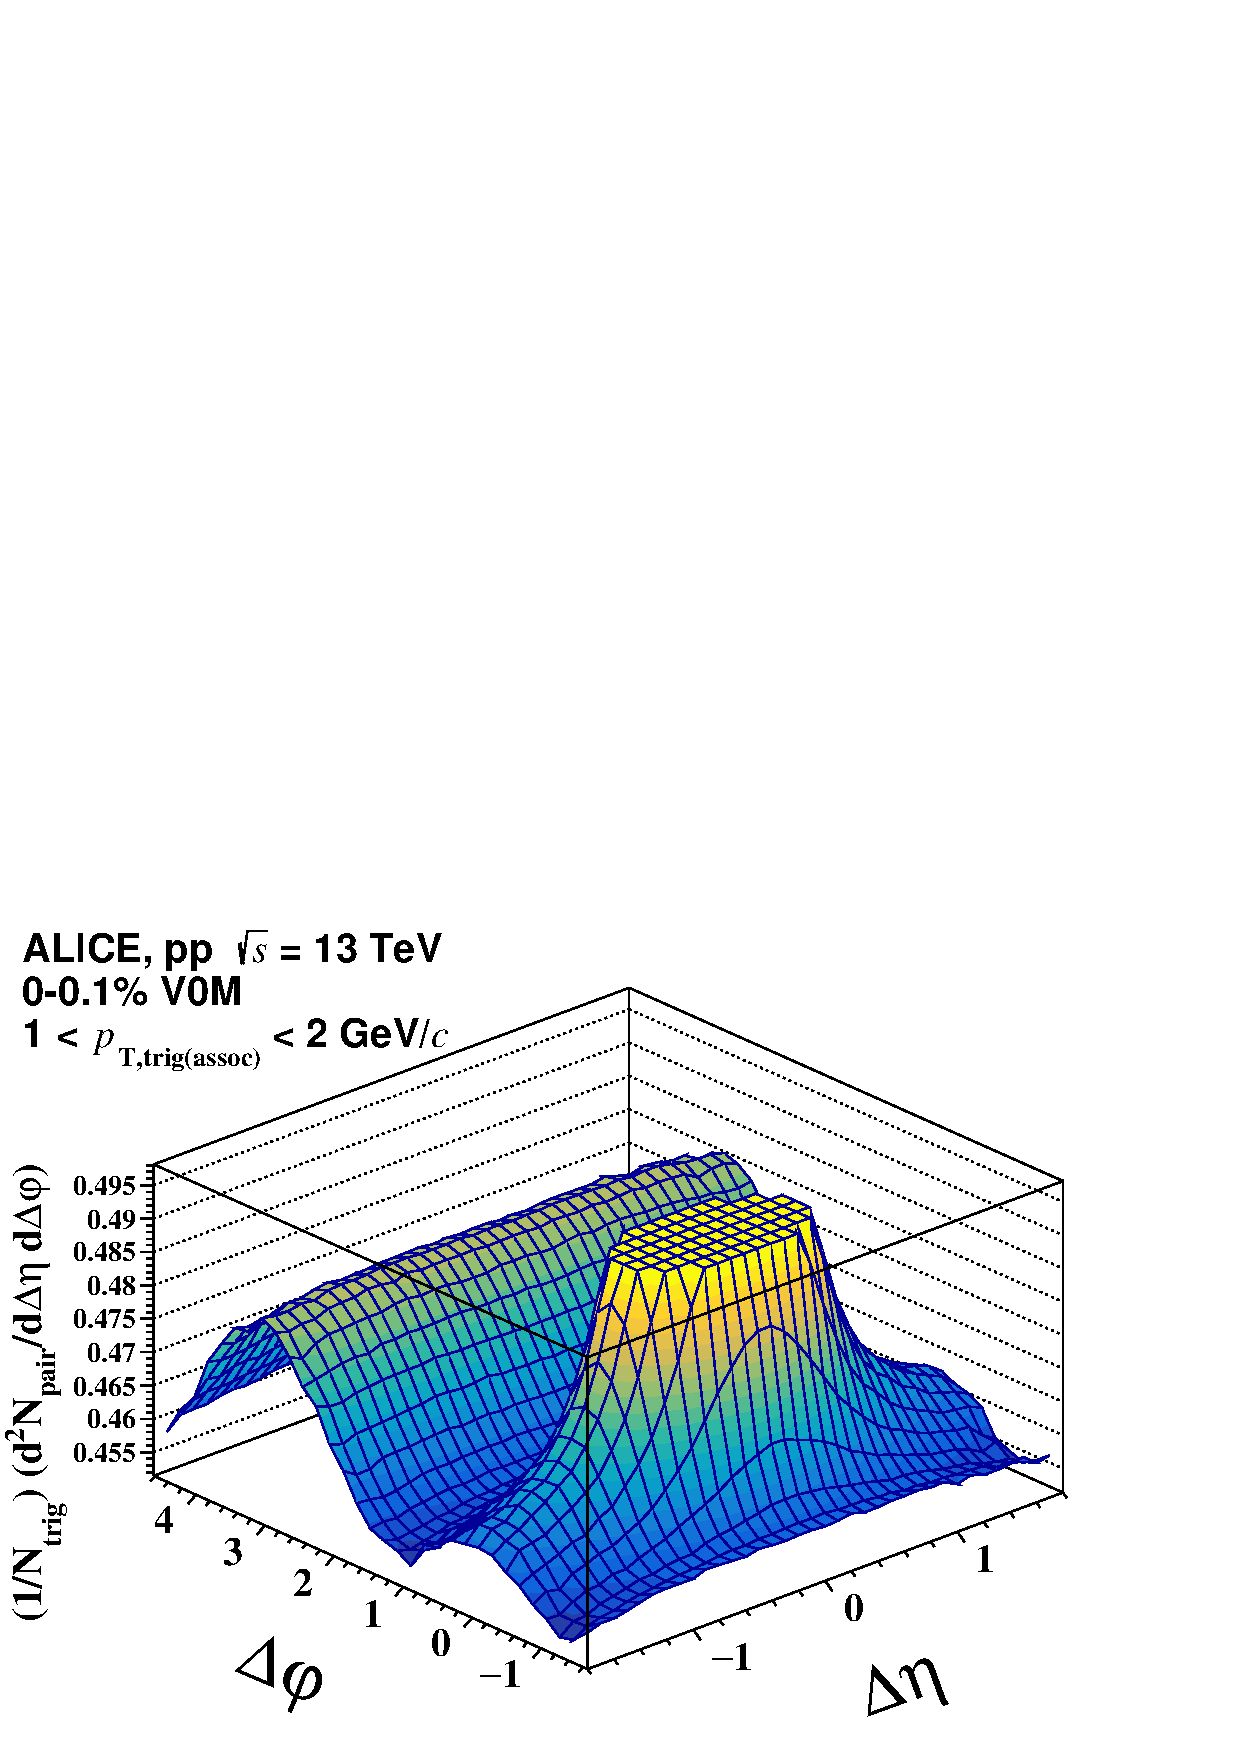
\includegraphics[width=0.47 \textwidth]{./figures/corr1.pdf} }
	\caption{ Two-particle correlation functions as functions of $\Delta\eta$ and $\Delta\varphi$ in minimum-bias events (0--100\%, left) and high-multiplicity (0--0.1\%, right). Note that the near-side jet peaks exceed the chosen range of the $z$-axis. The intervals of $\pttrig$ and $\ptassoc$ are 1~$<\it{p}_{\rm{T}}<$~2~GeV/$c$ in both cases.}
	\label{fig:PlotCorrMBHMT}
\end{figure}

Figure~\ref{fig:PlotCorrMBHMT} shows the per-trigger yield obtained from Eq.~(1) for 1~$<\pttrig~\mathrm (\ptassoc)<$~2 GeV/$c$ in pp collisions at $\sqrt{\it{s}} = $\unit{13} {\rm{}TeV} for minimum bias events (left) and high-multiplicity events (right). It is worth noting that the $z$-axes for the yield of the correlations is properly scaled in order to zoom in the ridge yield, as a result, the jet peaks are sheared off in both figures. The ridge structure is clearly observed in the high-multiplicity class while it is less significant in the minimum bias events. The away-side yield is populated mostly by back-to-back jet correlations.

\begin{figure}[h!]
	\centering
	\includegraphics[width=0.9\linewidth]{./figures/Fig2_PlotDeltaPhi.pdf}
	\caption{One-dimensional $\Delta\varphi$ distribution in the large $\Delta\eta$ projection for three transverse momentum intervals in minimum bias (upper panels) and high-multiplicity (lower panels) events after ZYAM subtraction. Transverse momentum intervals of the trigger particles and associated particles are 1~$<\pt<$~2 (left), 2~$<\pt<$~3 (middle) and, 3~$<\pt<$~4 GeV/$c$ (right), respectively. The presented model predictions were calculated using $\pythiashoving$, $\pythiam$, and $\epos$.}
	\label{fig:PlotDeltaPhi}
\end{figure}
 
Figure~\ref{fig:PlotDeltaPhi} shows $\Delta\varphi$ projections of the two-particle correlation functions obtained in the range 1.6~$<|\Delta \eta |<$~1.8 for several track $\pt$ intervals after the ZYAM subtraction (see Eq.~(2)). The results are shown for various $\it{p}_{\rm{T}}$ intervals in the minimum bias class (upper) and the high-multiplicity class (lower) down to 1~GeV/$c$ where the non-flow contamination is negligible. The near-side ($\Delta\varphi\sim 0$) ridge in the high-multiplicity class is clearly observed for $\pt<$~3~GeV/$c$ while there is no definitive signal in the minimum bias class. Within the range of analyzed particle $\pt$, the yield in the near-side ridge decreases with increasing $\pt$ in the high-multiplicity class.

The measurements in the high-multiplicity class are compared with the results published by the CMS Collaboration~\cite{Khachatryan:2015lva}. In case of the CMS measurement, the charged particle multiplicity was obtained by counting the number of particles satisfying $\pt>0.4$~GeV/$c$ in $|\eta|<$~2.4. In our analysis, event multiplicity is determined from the forward V0 detectors. The difference in multiplicity selection between ALICE (forward) and CMS (midrapidity) is studied using PYTHIA~8 simulations and it is found that the calculated multiplicity using the CMS procedure is about 20\% larger than the one from ALICE when compared in the acceptance region of the measurements reported in this article, $|\eta|<$~0.9. Near-side ridges in all transverse momentum ranges are comparable. The larger away-side yields observed in Fig.~\ref{fig:PlotDeltaPhi} for the CMS results can be attributed to the overlap in $\eta$ acceptance between the multiplicity selection and the correlation function measurement.

In Fig.~\ref{fig:PlotDeltaPhi}, the ALICE measurements are also compared with model predictions where a comparable high-multiplicity selection and $\Delta\eta$ projection range are applied. The selection of high-multiplicity events in the models is done by requiring a minimal number of charged particles emitted within the V0M detector acceptance. In case of $\pythiam$, the 0--0.1\% centrality threshold is 105 charged particles. The threshold for $\epos$ and $\pythiashoving$ are 110 and 108, respectively. The magnitude of string shoving ($g$) is set to 3.0 in this study. The statistical uncertainties due to the limited number of events for the model calculations are shown as bands in each figure. The $\pythiashoving$ provides good estimates of the near-side ridge yield and slightly overestimates the away-side yield for the interval 1~$<\it{p}_{\rm{T}}<$~2~GeV/$c$. However, the $\pythiashoving$ model underestimates the near-side ridge yield for $\it{p}_{\rm{T}}>$~2~GeV/$c$. The $\pythiam$ model does not show any near-side ridge as expected. It slightly underestimates the away-side peak for 1~$<\it{p}_{\rm{T}}<$~2~GeV/$c$ and provides good estimates for $\it{p}_{\rm{T}}>$~2~GeV/$c$. On the other hand, $\epos$ describes the shape of the ridge yield quantitatively better in the 2~$<\pttrigassoc<$~4~GeV/$c$ range, while overestimating the near-side ridge yield for $\pttrigassoc<$~2~GeV/$c$ range. 


\begin{figure}[h!]
	\centering
	\subfigure{\includegraphics[width=0.89\textwidth]{./figures/Fig3_PlotRidgeYield.pdf}}
	\caption{ Fully corrected near-side ridge yield as a function transverse momentum. The open blue boxes denote the measurement by ALICE. The statistical and systematic uncertainties are shown as vertical bars and boxes, respectively. The CMS measurement~\cite{Khachatryan:2015lva} is represented by filled circles and extends down to lower $\pt$ due to the larger $\Delta\eta$ acceptance. The three lines show model predictions from $\pythiam$ (blue dotted line), $\pythiashoving$ (orange line), and $\epos$ (green dashed line).}
	\label{fig:PlotYSpect}
\end{figure}

Figure~\ref{fig:PlotYSpect} shows the near-side ridge yield measured in high-multiplicity events as a function of $\pttrigassoc$. The measurement is compared with the result from CMS~\cite{Khachatryan:2015lva}.
%The ridge yields as a function of the transverse momentum are shown in Fig.~\ref{fig:PlotYSpect} in the high-multiplicity class and compared to \cite{Khachatryan:2015lva}.
Considering the differences in acceptance and the chosen multiplicity estimator of both measurements, perfect agreement between the two sets of results is not expected. The measurement is also compared with model calculations. As expected, the PYTHIA~8 model with Tune 4C does not produce a near-side ridge because it is not designed to account for this effect. The $\pythiashoving$ model describes the yield qualitatively, however the predicted yield decreases more rapidly than the measured one for increasing $\pttrigassoc$. The $\epos$ model, unlike the $\pythiashoving$ model, describes well the $\pt$ dependence of the ridge yield for the range $\it{p}_{\rm{T}}>$~2~GeV/$c$ , while predicting larger yields for $\it{p}_{\rm{T}}<$~2 GeV/$c$.

\subsection{Event-scale dependence of the ridge yield}
\begin{figure}[h!]
	\centering
	\subfigure{ 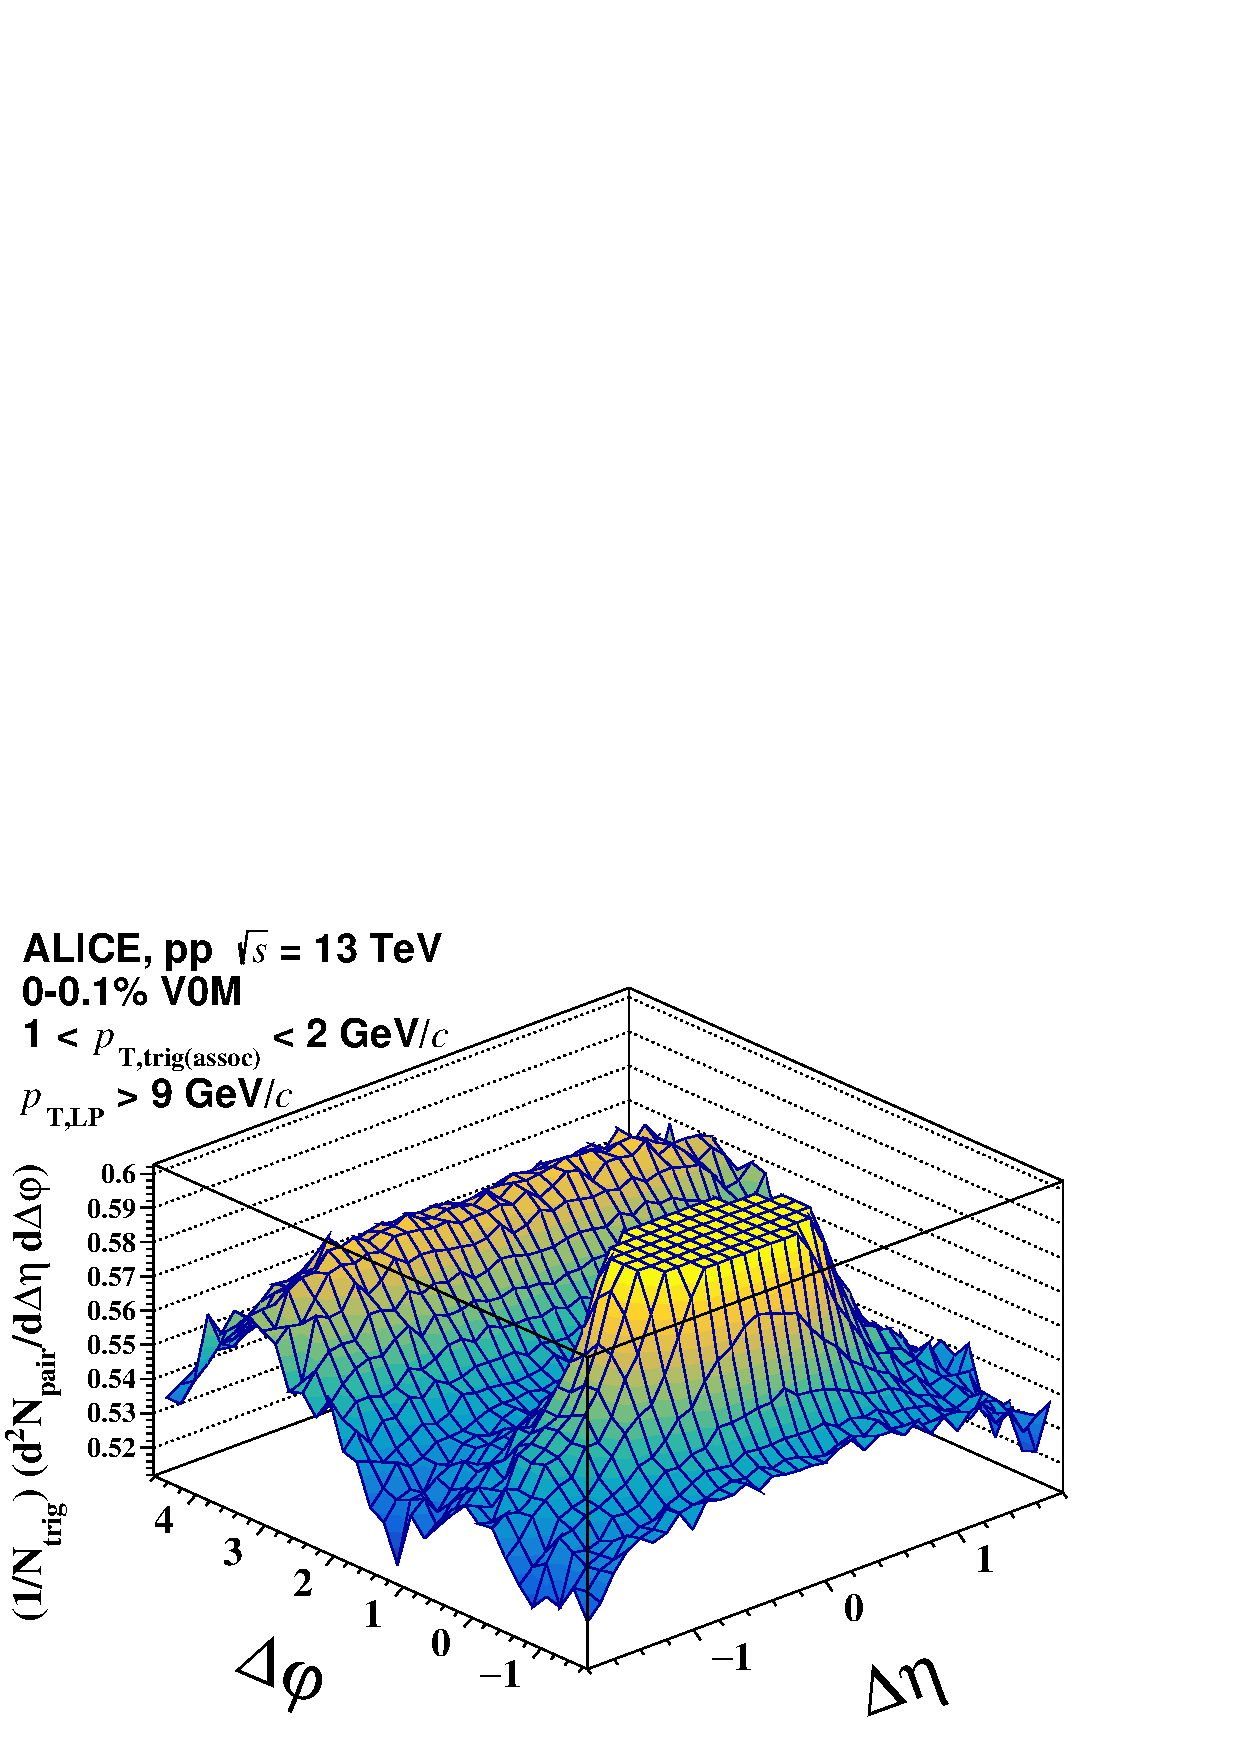
\includegraphics[width=0.47 \textwidth]{./figures/corrlh.pdf} }
	\subfigure{ 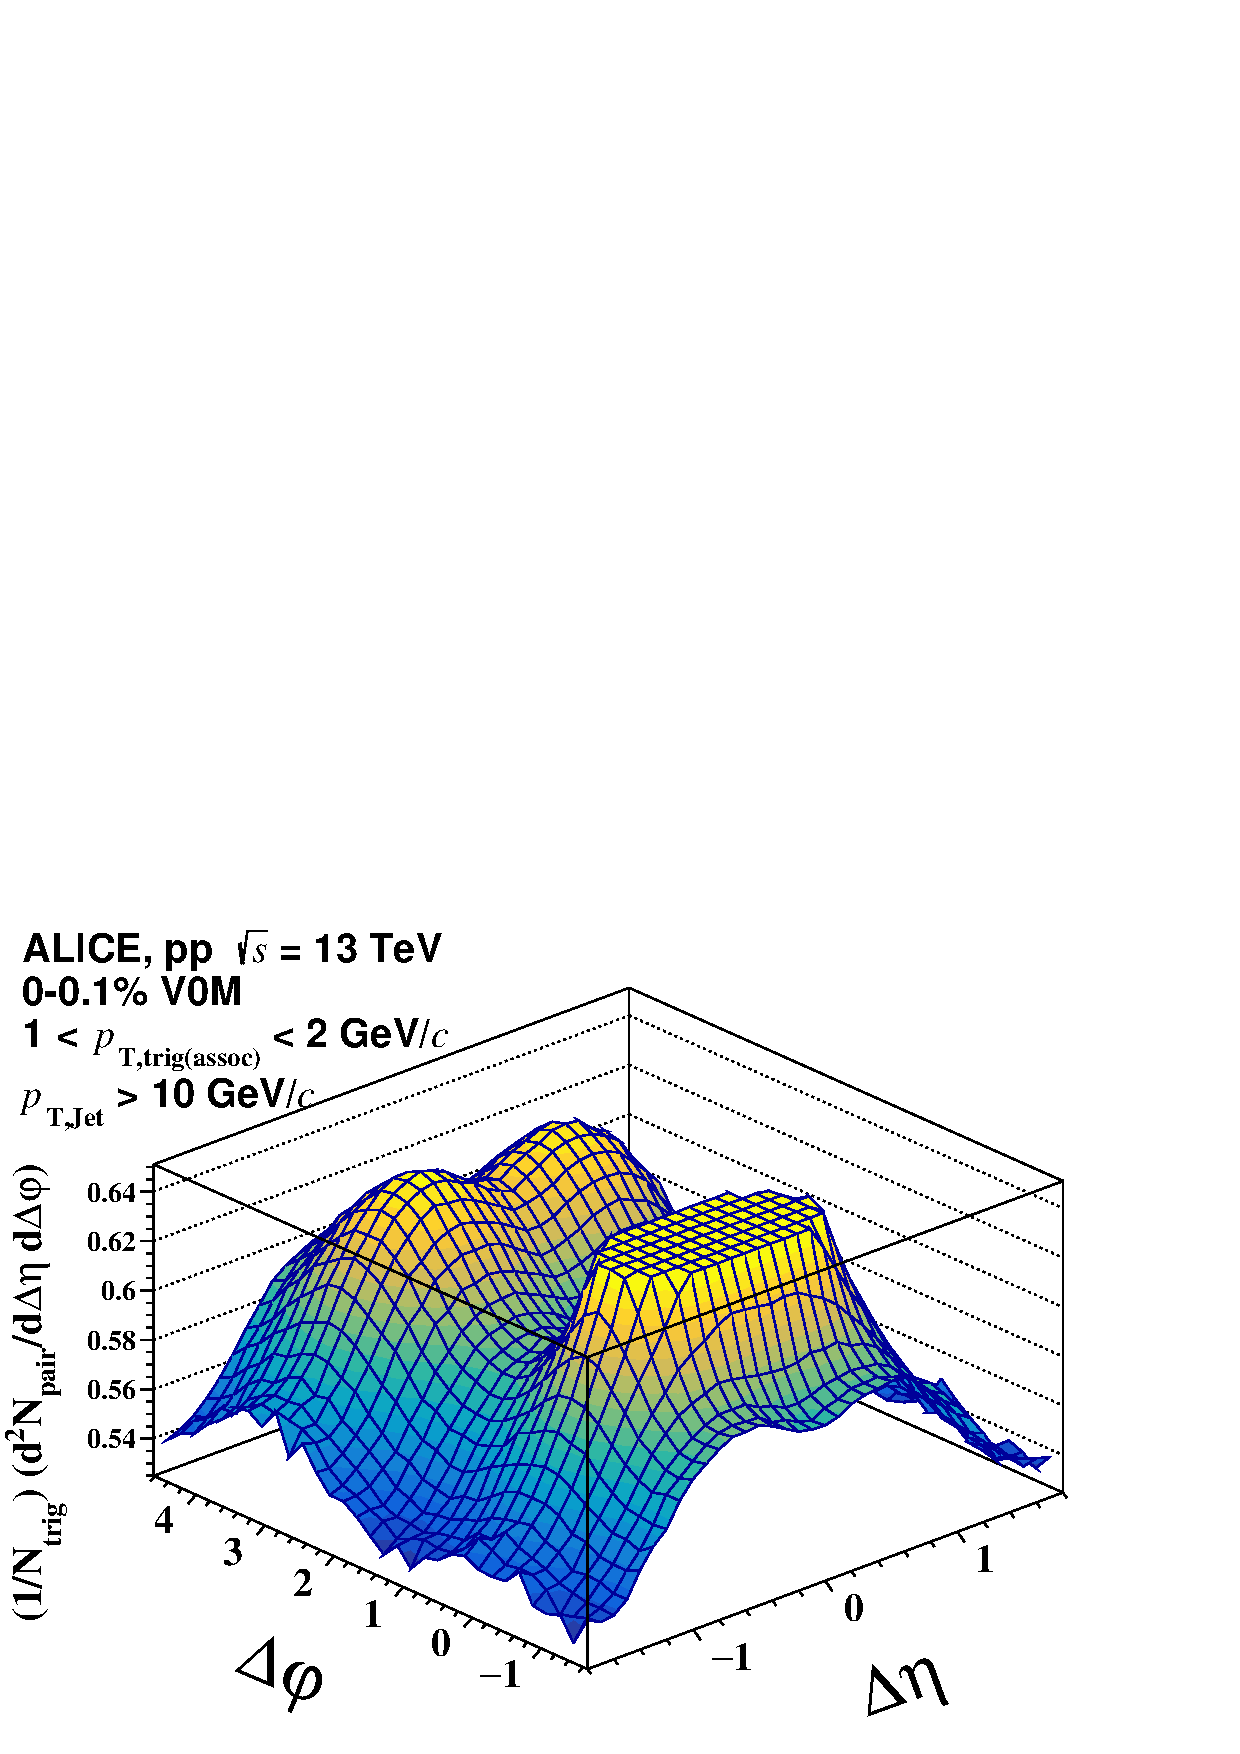
\includegraphics[width=0.47 \textwidth]{./figures/corrjet.pdf} }
	\caption{ Two-dimensional correlation functions as a function of $\Delta\eta$ and $\Delta\varphi$ in high-multiplicity events including a selection on the event-scale. The interval of $\pttrig$ and $\ptassoc$ is 1~$<\pttrigassoc<$~2~GeV/$c$. Left: HM events with a $\ptlead>$~9~GeV/$c$ leading track. Right: HM events with a $\ptjet>$~10~GeV/$c$.}
	\label{fig:PlotCorrHMTSel}
\end{figure}

The ridge yield is further studied with respect to two different event-scales. In the first measurement, the event-scale is set by requiring a minimum $\pt$ cutoff on the leading particle in each event (denoted as $\ptlead$), while in the second measurement, a minimum $\pt$ cutoff is imposed on the leading jet (denoted as $\ptjet$). 

Figure~\ref{fig:PlotCorrHMTSel} shows that the ridge structure for 1~$< \pttrig\,(\ptassoc) <$~2 GeV/$c$ still persists in high-multiplicity pp collisions with $\ptlead>$~9~GeV/$c$ (left) and $\ptjet>$~10~GeV/$c$ (right).  %The interval is the same to the measured ridge yield is maximum without the event-scale selection.
It is worth noting that the correlation function obtained with the minimum $\ptjet$ selection has a double peak structure which is oriented along the $\Delta\eta$ axis at $\Delta\varphi=\pi$. This structure emerges due to the restricted acceptance of the jet tagging, $|\eta_{\rm{jet}}|<$~0.4.

\begin{figure}[h!]
	\centering
	\includegraphics[width=0.99\linewidth]{./figures/Fig5_PlotDeltaPhiESE.pdf}
	\caption{ One-dimensional $\Delta\varphi$ projections of the correlation functions constrained to 1.6~$<|\Delta\eta|<$~1.8 in HM events with an additional event-scale bias. Top: with an imposed selection on the leading jet $\pt$,  bottom: with an imposed selection on the leading particle $\pt$. ALICE data are compared with prediction of models.}
	\label{fig:PlotDeltaPhiESE}
\end{figure}

Figure~\ref{fig:PlotDeltaPhiESE} shows projected $\Delta\varphi$ distributions of the correlation functions in 1.6~$<|\Delta\eta|<$~1.8 with the minimum $\ptlead$ (lower) and $\ptjet$ (upper) requirement. Even with the event-scale selection, the ridge is still visible on the near-side. The near-side ridge peak increases as the thresholds of $\ptlead$ and $\ptjet$ increase compared to the one measured in unbiased events in Sec.~\ref{sec:resultunbiased}. The results are compared with $\pythiashoving$, $\pythiam$, and $\epos$ calculations. The near-side ridge peaks are qualitatively reproduced by $\pythiashoving$ and $\epos$ models. On the other hand, the $\pythiam$ does not show the  near-side ridge peak for neither of the two event-scale selections, but it gives compatible results for the away-side yield just like the $\pythiashoving$ model.

%Both models describe the away-side yield with the $\ptjet$ selection and overestimate away-side yield with the $\ptlead$ selection.

\begin{figure}[h!]
	\centering
	\includegraphics[width=0.89\linewidth]{./figures/Fig6_RidgeYieldESE.pdf}
	\caption{Near-side ridge yield as a function of the $\it{p}^{\rm{LP}}_{\rm{T,min}}$ (left) and $\it{p}^{\rm{Jet}}_{\rm{T,min}}$ (right). Data points (filled circles) show the ALICE measurement. The statistical and systematic uncertainties are shown as vertical bars and boxes, respectively. As the ridge yield is obtained in the same operational way for data and models, the upper limit of the systematic uncertainty due to jet contamination, which is 18.9\%, is not included in the figure. The data are compared with predictions of models which are represented by colored bands. The bottom panel shows a ratio of the models to the data. The uncertainty of the data is represented by the gray band centered around unity.}
	\label{fig:RidgeYield_ESE}
\end{figure}

The ridge yields as function of the minimum $\ptlead$ ($\it{p}^{\rm{LP}}_{\rm{T,min}}$) and $\ptjet$ ($\it{p}^{\rm{jet}}_{\rm{T,min}}$) selections are shown in Fig.~\ref{fig:RidgeYield_ESE}. High-multiplicity events with imposed event-scale bias exhibit increased ridge yields when compared to unbiased HM events. A small increase of the ridge yields as a function of $\ptlead$ or $\ptjet$ is observed and there is no difference between the two event-scale selections within the uncertainties. Comparisons to model calculations show that $\pythiashoving$ provides a comparable trend with data, but underestimates the ridge yield. On the other hand, $\epos$ overestimates the ridge yield while providing a trend comparable with the data. The origin of the enhanced ridge yields for higher momentum jet-tagged events is not clear to date but it might be related to the expected smaller impact parameters for dijet or multi-jet production events as studied in~\cite{Frankfurt:2010ea}.

\begin{figure}[h!]
	\centering
	\includegraphics[width=0.89\linewidth]{./figures/Fig9_JetYieldESE.pdf}
	\caption{ Near-side jet-like peak yield as a function of the $\it{p}^{\rm{LP}}_{\rm{T,min}}$ (left) and $\it{p}^{\rm{jet}}_{\rm{T,min}}$ (right). The filled circles show measurement with ALICE. The statistical and systematic uncertainties are shown as vertical bars and boxes, respectively. The measurements are compared with model descriptions from $\pythiam$, $\pythiashoving$, and $\epos$ for both selections. The total uncertainty of the ratio is represented by the gray band centered around unity.}
	\label{fig:JetYield_ESE}
\end{figure}

Finally, the near-side jet-like peak yield is measured as a function of minimum $\ptlead$ and $\ptjet$ in Fig.~\ref{fig:JetYield_ESE} to further test the models that aim to describe the near-side ridge. $\epos$ provides comparable estimates of the near-side jet-like peak yield, while $\pythiam$ and $\pythiashoving$ overestimate the near-side yields for both event selections.

In all models if the ridge is due to final-state interactions, e.g., $\epos$ and PYTHIA~8 String Shoving, one also expects the near-side jet-like peak yield to be affected. This can be observed when comparing the measured near-side jet yields with PYTHIA~8 calculations with and without String Shoving. The new ALICE results therefore provide constraints beyond traditional ridge measurements that challenge existing models.
% !TEX root = paper.tex

\section{Conclusions}
\label{sec:summary}

Long- and short-range correlations for pairs of charged particles with 1$ < \pt < $4~GeV/$c$ have been studied in pp collisions at $\sqrt{s} = 13$~TeV with a focus on high-multiplicity events. The ridge and near-side jet yields have been extracted and their event scale dependence have been studied. The obtained long-range ridge yields are compatible with the measurements by the CMS collaboration~\cite{Khachatryan:2015lva}.
%In addition, the $\pt$ and the $\it{p}_{\rm{T,Lead}}$ or $\it{p}_{\rm{T,Jet}}$ selection dependence of the long-range azimuthal correlations are measured.
$\pythiashoving$ describes the yield qualitatively but the predicted yield decreases more rapidly than the data as $\pttrigassoc$ increases. On the other hand, $\epos$ gives better description for $\pt$ dependence while overestimating the ridge yield for $\pt<$2 GeV/$c$. Finally, no long-range ridge is formed in $\pythiam$.
%Furthermore the ridge yields are studied in events, where jets with a harder fragmentation are preferred by requiring the minimum value of the transverse momentum of leading particles in each event $\ptlead$ or the one of reconstructed jets $\ptjet$. The ridge structure still persist with both selections. The ridge yields increase as $\ptlead$ and $\ptjet$ increase. The latter, however, is more significant than the former selection. The results are compared with $\pythiashoving$ calculations, showing the enhancement while underestimating the absolute ridge yield.
The ridge yields were further studied in high-multiplicity events biased with additional event scale selections, which imposed a minimum transverse momentum cutoff on a leading track or jet. The ridge structure still persists with both selections. The ridge yields increase as $\ptlead$ and $\ptjet$ increase. The results are compared with $\pythiashoving$, $\epos$ and $\pythiam$ calculations. $\pythiashoving$ and $\epos$ estimate qualitatively the trends for event-scale selection. However, the former underestimates the ridge yield and the latter overestimates the ridge yield. The models are further tested whether they reproduce the yield of the near-side jet-like correlation measured in the biased events.

Evolution of the near-side jet yield as a function event-scale $\pt$ is better captured by $\epos$, while $\pythiashoving$ tends to overshoot the data. 
%which results in opposite trends between the ridge yield and near-side jet-like correlations.
The results might open new way of studying impact parameter dependence of the small systems with jet tagged events in the future and will help to explore possible physical origins of long-range correlations.


%%%%% acknowledgements
\newenvironment{acknowledgement}{\relax}{\relax}
\begin{acknowledgement}
\section*{Acknowledgements}
\noindent The ALICE Collaboration would like to thank Christian Bierlich for providing the PYTHIA8 string shoving calculations.
%{\it (TBI: The default acknowledgments will be done by EB centrally.)}
%\input{acknowledgements.tex}    %%%%%%% done by webmaster team
\end{acknowledgement}

\newpage
\appendix



\clearpage

\bibliographystyle{utphys}
\bibliography{paper.bib}

%%%%%%%%% appendix with author list
%\section{The ALICE Collaboration}
%\label{app:collab}
%\input{Alice_Authorlist_2017-Aug-21.tex}  %%%%%%% done by webmaster team
%\input{}     


\end{document}